\documentclass[xcolor={dvipsnames,table}]{beamer}
\usepackage{epsfig,graphicx}
\usepackage{palatino}
\usepackage{fancybox}
\usepackage{relsize}
\usepackage[procnames]{listings}
\usepackage{hyperref}
\usepackage{qtree} % needed?
\usepackage{booktabs}
\usepackage{dirtree}
\usepackage[normalem]{ulem}
\usepackage{tikz}
\usetikzlibrary{arrows.meta,positioning,calc,fit,shapes.geometric,decorations.pathreplacing}


% fatter TT font
\renewcommand*\ttdefault{txtt}
% another TT, suggested by Alex
% \usepackage{inconsolata}
% \usepackage[T1]{fontenc} % needed as well?


\newcommand{\scale}{0.7}

\newcommand{\todo}[1]{{\emph{TODO: #1}}}
\newcommand{\martin}[1]{{\color{blue} Martin: #1}}
\newcommand{\abcdef}[1]{{\color{red} Author2: #1}}

% uncomment following for final submission
%\renewcommand{\todo}[1]{}
%\renewcommand{\martin}[1]{}
%\renewcommand{\author2}[1]{}

\newcommand{\code}[1]{{\texttt{#1}}}

\hypersetup{
  linkcolor  = black,
%  citecolor  = blue,
  urlcolor   = blue,
  colorlinks = true,
}

\beamertemplatenavigationsymbolsempty
\setbeamertemplate{footline}[frame number]





\newif\ifbook
\input{../shared/chisel}

% TikZ for diagrams
\usepackage{tikz}
\usetikzlibrary{positioning, arrows.meta}

% Optional visual tweaks
\tikzset{
    >=Stealth,
    every node/.style={rounded corners=2pt}
}

\title{Introduction to Agile and Scala}
\author{Martin Schoeberl}
\date{\today}
\institute{Technical University of Denmark\\
Embedded Systems Engineering}

\begin{document}

\begin{frame}
\titlepage
\end{frame}




\begin{frame}[fragile]{Outline}
\begin{itemize}
\item Waterfall and Agile design style
\item Introduction to Scala
\item Functional programming in Scala
\item Links to further reading and material
\end{itemize}
\end{frame}

% Week 1: Intro to Agile + Chisel

% --- Slide 1: Waterfall Model (Description) ---
\begin{frame}{The Classic Waterfall Model}
\begin{itemize}
    \item Traditional project management approach for software and hardware
    \item Development phases are sequential:
    \begin{enumerate}
        \item Requirements
        \item Design
        \item Implementation
        \item Verification
        \item Maintenance
    \end{enumerate}
    \item Each phase must be completed before moving to the next
    \item Changes are costly once early phases are complete
    \item I worked (long time ago) in such a team: was very boring
\end{itemize}
\end{frame}

\begin{frame}{Waterfall Model Diagram}
\centering
\resizebox{0.8\linewidth}{!}{%
\begin{tikzpicture}[
    node distance=1.4cm,
    every node/.style={draw, minimum width=3.2cm, minimum height=1.2cm, align=center}
]
\node[thick] (req) {Requirements};
\node[thick] (design) [below right=0.8cm and 0.6cm of req] {Design};
\node[thick] (impl) [below right=0.8cm and 0.6cm of design] {Implementation};
\node[thick] (verif) [below right=0.8cm and 0.6cm of impl] {Verification};
\node[thick] (maint) [below right=0.8cm and 0.6cm of verif] {Maintenance};

% Arrows
\draw[->, thick] (req.south east) -- (design.north west);
\draw[->, thick] (design.south east) -- (impl.north west);
\draw[->, thick] (impl.south east) -- (verif.north west);
\draw[->, thick] (verif.south east) -- (maint.north west);

% Feedback arrows
\draw[->, dashed, red] (design.west) .. controls +( -2,0) and +(-2,0) .. (req.west) node[midway,left]{Costly change};
\draw[->, dashed, red] (impl.west) .. controls +( -2,0) and +(-2,0) .. (design.west);
\draw[->, dashed, red] (verif.west) .. controls +( -2,0) and +(-2,0) .. (impl.west);

\end{tikzpicture}%
}
\end{frame}

% --- Slide 3: Waterfall Limitations ---
\begin{frame}{Limitations of the Waterfall Model}
\begin{itemize}
    \item Assumes requirements are fixed at the start
    \item Poor adaptability to changing customer needs
    \item Testing and feedback happen late in the process
    \item High risk of discovering major flaws late
    \item Not well-suited for rapid prototyping or exploratory projects
    \item Worked at Compaq for a banking SW in this style
\end{itemize}
\end{frame}


\begin{frame}{Why Agile for Hardware?}
\begin{itemize}
    \item Traditional hardware development: long, rigid cycles
    \item Software has embraced Agile:
    \begin{itemize}
        \item Quick iterations
        \item Test-driven development
        \item Continuous integration
    \end{itemize}
    \item Hardware complexity is increasing $\rightarrow$ need for agility!
\end{itemize}
\end{frame}

\begin{frame}{Agile Iteration Cycle}
\centering
\resizebox{0.65\linewidth}{!}{%
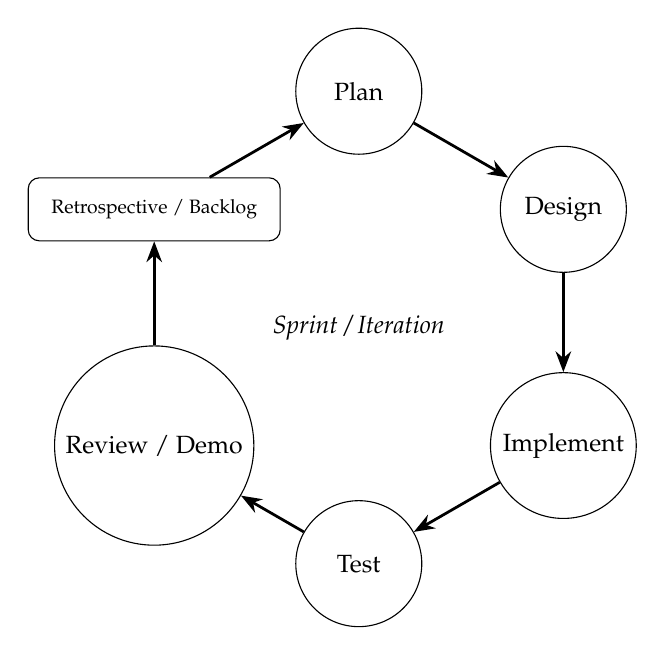
\begin{tikzpicture}[
  circular/.style={circle, draw, minimum size=1.6cm, font=\small, align=center},
  arrowstyle/.style={-Stealth, line width=1pt}
]
  % Place nodes in a circular layout
  \node[circular] (plan)      at (90:3cm)  {Plan};
  \node[circular] (design)    at (30:3cm)  {Design};
  \node[circular] (implement) at (-30:3cm) {Implement};
  \node[circular] (test)      at (-90:3cm) {Test};
  \node[circular] (review)    at (-150:3cm) {Review / Demo};
  \node[rectangle, draw, rounded corners, minimum width=3.2cm, minimum height=0.8cm, font=\scriptsize] (retro) at (-210:3cm) {Retrospective / Backlog};

  % Loop arrows
  \draw[arrowstyle] (plan) -- (design);
  \draw[arrowstyle] (design) -- (implement);
  \draw[arrowstyle] (implement) -- (test);
  \draw[arrowstyle] (test) -- (review);
  \draw[arrowstyle] (review) -- (retro);
  \draw[arrowstyle] (retro) -- (plan);

  % Central label
  \node at (0,0) [font=\small\itshape] {Sprint / Iteration};
\end{tikzpicture}%
}
\end{frame}

\begin{frame}{Agile Iteration Phases (1/3)}
\textbf{Plan}
\begin{itemize}
    \item Define goals for the upcoming sprint (typically 1-4 weeks)
    \item Select features or fixes from the product backlog
    \item Break down tasks into manageable user stories
    \item Ensure each story has clear acceptance criteria
\end{itemize}

\medskip
\textbf{Design}
\begin{itemize}
    \item Create a simple, implementable hardware design
    \item Define interfaces and parameters
    \item Update documentation and diagrams
    \item Keep the design minimal to support fast iteration
    \item Think: minimal viable product
\end{itemize}
\end{frame}

% --- Slide 2 ---
\begin{frame}{Agile Iteration Phases (2/3)}
\textbf{Implement}
\begin{itemize}
    \item Write Chisel modules for new or updated functionality
    \item Commit early and often to version control
    \item Follow coding standards and naming conventions
    \item Collaborate closely to avoid merge conflicts
\end{itemize}

\medskip
\textbf{Test}
\begin{itemize}
    \item Use automated tests (e.g., \texttt{chiseltest}) to validate functionality
    \item Run both unit tests and integration tests
    \item Include corner cases and property-based checks
    \item Maintain high test coverage throughout development
\end{itemize}
\end{frame}

% --- Slide 3 ---
\begin{frame}{Agile Iteration Phases (3/3)}
\textbf{Review / Demo}
\begin{itemize}
    \item Present completed work to the team or stakeholders
    \item Demonstrate working features in simulation or on FPGA
    \item Gather feedback on design choices and implementation
\end{itemize}

\medskip
\textbf{Retrospective / Backlog Refinement}
\begin{itemize}
    \item Reflect on what worked well and what can be improved
    \item Adjust processes, tools, and team coordination as needed
    \item Update the product backlog with new ideas or changes
    \item Prepare for the next sprint cycle
\end{itemize}
\end{frame}

\begin{frame}[fragile]{XXX}
\begin{itemize}
\item xxx
\item xxx
\item xxx
\item xxx
\item xxx
\end{itemize}
\end{frame}

\begin{frame}{Hardware Design Today}
\begin{itemize}
    \item VHDL / Verilog = rigid, low-level
    \item Hard to reuse and test modularly
    \item Long simulation cycles
    \item Not optimized for iteration or testing early
    \item Often follows a version of the waterfall model
\end{itemize}
\end{frame}

\begin{frame}{Software-Inspired Hardware Flow}
\begin{enumerate}
    \item Write modular, parameterized designs
    \item Test-first using simulation
    \item Version control and continuous integration (CI)
    \begin{itemize}
\item For example, using GitHub actions
\end{itemize}
    \item Frequent review and refactor
    \begin{itemize}
\item With enough tests, refactoring is safe
\end{itemize}
    \item Code reviews and pull requests
\end{enumerate}
\end{frame}


\begin{frame}[fragile]{What Language do You Already Know?}
\begin{itemize}
\item Python
\item Java
\item C
\item Scala
\item VHDL
\item Verilog
\item Chisel
\item Haskell
\item Clash
\item Other
\end{itemize}
\end{frame}

\begin{frame}[fragile]{On Chisel}
\begin{itemize}
\item The course will use Chisel and Scala
\item Next week, 1 hour intro to Chisel
\item If you know it already, join at 14:00
\item Start reading the Chisel book
\end{itemize}
\end{frame}

\begin{frame}[fragile]{A Chisel Book}
\begin{figure}
    \centering
    \href{https://github.com/schoeberl/chisel-book}{\includegraphics[scale=0.4]{../cover-small}}
\end{figure}

\begin{itemize}
\item Available in open access (\href{https://www.imm.dtu.dk/~masca/chisel-book.pdf}{as PDF})
\begin{itemize}
\item Optimized for reading on a tablet (size, hyperlinks)
\end{itemize}
\item Amazon can do the printout
\end{itemize}
\end{frame}

\begin{frame}[fragile]{Scala}
\begin{itemize}
\item Object-oriented
\item Functional
\item Strongly typed with very good type inference
\item Runs on the Java virtual machine
\item Can call Java libraries
\item Consider it as Java++
\begin{itemize}
\item Can almost be written like Java
\item With a more lightweight syntax
\item Compiled to the JVM
\item Good Java interoperability
\item Many libraries available
\end{itemize}
\item \url{https://docs.scala-lang.org/tour/tour-of-scala.html}
\end{itemize}
\end{frame}

\begin{frame}[fragile]{Scala Hello World}
\begin{chisel}
object HelloWorld extends App {
  println("Hello, World!")
}
\end{chisel}
\begin{itemize}
\item Compile with \code{scalac} and run with \code{scala}
\item Or with \code{sbt run}
\item You can even use Scala as a scripting language
\item \code{scala-cli} is a generic Scala runner
\item Show both
\item Use \code{scala-cli} locally along the examples presented
\end{itemize}
\end{frame}

\begin{frame}[fragile]{The ``Real'' Hello World}

\begin{verbatim}
object Hello {
  def main(args: Array[String]): Unit = {
    println("Hello, world!")
  }
}
\end{verbatim}

\begin{itemize}
    \item Every program starts with an \texttt{object} and a \texttt{main} method
    \item Use \texttt{println} to print to the console
    \item Access to command line arguments via \code{args}
    \item Similar ot the Java static \code{main} function
\end{itemize}
\end{frame}

\begin{frame}[fragile]{Scala Values and Variables}
\begin{itemize}
    \item Scala distinguishes between immutable (\texttt{val}) and mutable (\texttt{var})
    \item By default, use \texttt{val} (immutability is preferred)
\end{itemize}
\begin{chisel}
// A value is a constant
val i = 0
// No new assignment; this will not compile
i = 3

// A variable can change the value
var v = "Hello"
v = "Hello World"

// Type usually inferred, but can be declared
var s: String = "abc"
\end{chisel}
\end{frame}

\begin{frame}[fragile]{Basic Types}
\begin{itemize}
    \item Common Scala types:
\end{itemize}

\begin{verbatim}
val a: Int = 42
val b: Double = 3.14
val c: Boolean = true
val d: String = "Scala"
\end{verbatim}

\begin{itemize}
    \item Type inference: Scala often figures out the type for you
\end{itemize}

\begin{verbatim}
val x = 100     // Int
val y = "hi"    // String
\end{verbatim}
\end{frame}

\begin{frame}[fragile]{Simple Loops}
\begin{chisel}
// Loops from 0 to 9
// Automatically creates loop value i
for (i <- 0 until 10) {
  println(i)
}
\end{chisel}
\end{frame}

\begin{frame}[fragile]{Conditions}
\begin{chisel}
for (i <- 0 until 10) {
  if (i%2 == 0) {
    println(i + " is even")
  } else {
    println(i + " is odd")
  }
}
\end{chisel}
\end{frame}

\begin{frame}[fragile]{Expressions and Functions}
\begin{itemize}
    \item Everything in Scala is an expression (returns a value)
\end{itemize}

\begin{verbatim}
val sum = 1 + 2   // 3
val cond = if (sum > 2) "big" else "small"
\end{verbatim}

\begin{itemize}
    \item Defining a function:
\end{itemize}

\begin{verbatim}
def add(a: Int, b: Int): Int = {
  a + b
}
\end{verbatim}
\end{frame}


\begin{frame}[fragile]{Scala Arrays and Lists}
\begin{chisel}
// An integer array with 10 elements
val numbers = new Array[Integer](10)
for (i <- 0 until numbers.length) {
  numbers(i) = i*10
}
println(numbers(9))


// List of integers
val list = List(1, 2, 3)
println(list)
// Different form of list construction
val listenum = 'a' :: 'b' :: 'c' :: Nil
println(listenum)
\end{chisel}
\end{frame}

\begin{frame}[fragile]{Scala Collections}
\begin{itemize}
\item Scala has a powerful \href{https://docs.scala-lang.org/overviews/collections-2.13/overview.html}{collection library}
\item \code{Seq} is an ordered collection of elements (also called a sequence)
\item The default implementation is immutable
\item We index into a \code{Seq} with \code{()}, with zero-based indexing
\item Collections work well with functional programming
\end{itemize}
\shortlist{../code/scala_seq.txt}
\end{frame}

\begin{frame}[fragile]{Lists}
\begin{itemize}
    \item Lists are common in Scala
    \item Default list is immutable
\end{itemize}

\begin{verbatim}
val nums = List(1, 2, 3, 4)

// head and tail
println(nums.head)  // 1
println(nums.tail)  // List(2, 3, 4)

// append
val nums2 = nums :+ 5
\end{verbatim}

\begin{itemize}
\item When you append to a List it creats a new list
\end{itemize}
\end{frame}

\begin{frame}[fragile]{Scala Classes}
\begin{chisel}
// A simple class
class Example {
  // A field, initialized in the constructor
  var n = 0
  
  // A setter method
  def set(v: Integer) = {
    n = v
  }
  
  // Another method
  def print() = {
    println(n)
  }
}
\end{chisel}
\end{frame}

\begin{frame}[fragile]{Scala (Singleton) Object}
\begin{chisel}
object Example {}
\end{chisel}
\begin{itemize}
\item For \emph{static} fields and methods
\begin{itemize}
\item Scala has no static fields or methods like Java
\end{itemize}
\item Needed for \code{main}
\item Useful for helper functions
\end{itemize}
\end{frame}

\begin{frame}[fragile]{Tuples}
\begin{itemize}
\item Scala has the notion of tuples
\item Can hold a sequence of different types
\item Fields are then accessed with \code{.\_n}, starting with 1
\item Easy option to return more than one value from a function
\end{itemize}
\shortlist{../code/scala_tuple.txt}
\end{frame}



\begin{frame}[fragile]{Functional Programming}
\begin{itemize}
\item Functional programming (FP) treats computation as the evaluation of functions
\item Functions are first-class objects
\item Can be a parameter of a function
\item Can be returned from a function
\item Avoid mutable state
\item Recursion is \emph{not} the main point of FP
\item Higher-order functions take functions as arguments
\end{itemize}
\end{frame}


\begin{frame}[fragile]{First-Class Functions}
\begin{itemize}
    \item In Scala, functions can be assigned to variables, passed as arguments, or returned
\end{itemize}

\begin{verbatim}
// A normal function definition
def double(x: Int): Int = x * 2

println(double(5))   // prints 10

// A function that takes another function
def applyTwice(f: Int => Int, v: Int): Int = {
  f(f(v))
}

println(applyTwice(double, 3)) // prints 12
\end{verbatim}
\end{frame}

\begin{frame}[fragile]{Function Literals (Anonymous Functions)}
\begin{itemize}
    \item A function literal is a shorthand for defining a function "inline"
    \item by the \code{=>} symbol
    \item Does not require a name (\texttt{def})
    \item Often used with higher-order functions
\end{itemize}

\begin{verbatim}
// Normal function
def square(x: Int): Int = x * x

// Function literal (anonymous function)
val squareFn = (x: Int) => x * x

// Using a literal directly
val nums = List(1, 2, 3, 4)
val squares = nums.map(x => x * x)
println(squares) // List(1, 4, 9, 16)
\end{verbatim}
\end{frame}

% --- Slide 3 ---
\begin{frame}[fragile]{Higher-Order Functions}
\begin{itemize}
    \item Functions that take other functions as arguments
    \item What we just used before
    \item Useful for hardware generators (map, filter, etc.)
\end{itemize}

\begin{verbatim}
val nums = List(1, 2, 3, 4)
val squares = nums.map(x => x * x)
println(squares) // List(1, 4, 9, 16)
\end{verbatim}

%\begin{itemize}
%    \item This is similar to generating a Vec of wires in Chisel:
%\end{itemize}
%
%\begin{verbatim}
%val wires = VecInit(Seq.fill(4)(Wire(UInt(8.W))))
%\end{verbatim}
\end{frame}

% --- Slide 4 ---
\begin{frame}[fragile]{Immutability}
\begin{itemize}
    \item FP encourages immutable values (using \texttt{val})
    \item No side effects: easier to reason about hardware generation
\end{itemize}

\begin{verbatim}
val a = 5
// a = 6   // ERROR: reassignment not allowed

val b = a + 1   // OK, creates a new value
\end{verbatim}

\begin{itemize}
    \item In Chisel, \texttt{val} describes structure, not time-varying state
    \item Registers (\texttt{Reg}) are explicit when you need mutable hardware state
\end{itemize}
\end{frame}

% --- Slide 5 ---
%\begin{frame}[fragile]{Pure Functions}
%\begin{itemize}
%    \item A pure function:
%    \begin{itemize}
%        \item Always returns the same output for the same input
%        \item Has no side effects
%    \end{itemize}
%\end{itemize}
%
%\begin{verbatim}
%def add(a: Int, b: Int): Int = a + b
%\end{verbatim}
%
%\begin{itemize}
%    \item Combinational hardware modules are pure
%    \item Side effects (state, IO, randomness) are controlled explicitly
%\end{itemize}
%\end{frame}

% --- Slide 6 ---
\begin{frame}[fragile]{Mapping Over Collections}
\begin{itemize}
    \item \texttt{map} applies a function to each element of a collection
    \item Produces a new collection of the same size
\end{itemize}

\begin{verbatim}
val nums = List(1, 2, 3, 4)
def square(x: Int): Int = x * x

val squares = nums.map(square)
println(squares) // List(1, 4, 9, 16)
\end{verbatim}

\end{frame}

% --- Slide 7 ---
\begin{frame}[fragile]{Filtering Collections}
\begin{itemize}
    \item \texttt{filter} keeps only elements that satisfy a condition
\end{itemize}

\begin{verbatim}
val nums = List(1, 2, 3, 4, 5, 6)

def isEven(x: Int): Boolean = (x % 2 == 0)
val evens = nums.filter(isEven)

println(evens) // List(2, 4, 6)
\end{verbatim}

\end{frame}

% --- Slide 8 ---
\begin{frame}[fragile]{Reducing Collections}
\begin{itemize}
    \item \texttt{reduce} combines all elements using a binary function
    \item Useful for sums, products, and combining signals
\end{itemize}

\begin{verbatim}
val nums = List(1, 2, 3, 4)

def add(x: Int, y: Int): Int = x + y
val sum = nums.reduce(add)

println(sum) // 10
\end{verbatim}

\begin{itemize}
    \item Hardware analogy: adding a set of signals
    \item Use \code{reduceTree} for a balanced reduction tree
\end{itemize}
\end{frame}



\begin{frame}[fragile]{Scala Build Tool (sbt)}
\begin{itemize}
\item Downloads Scala compiler if needed
\item Downloads dependent libraries (e.g., Chisel)
\item Compiles Scala programs
\item Executes Scala programs
\item Does a lot of magic, maybe too much
\item Compile and run with:
\end{itemize}
\begin{chisel}
sbt run
\end{chisel}
\end{frame}

\begin{frame}[fragile]{File Organization in Scala/Chisel}
\dirtree{%
.1 project.
.2 src.
.3 main.
.4 scala.
.5 package.
.6 sub-package.
.3 test.
.4 scala.
.5 package.
.2 target.
.2 generated.
}
\end{frame}



\begin{frame}[fragile]{ScalaTest}
\begin{itemize}
\item Testing framework for Scala and Java
\item \code{sbt} understands ScalaTest
\item Add library to \code{build.sbt}
\begin{chisel}
libraryDependencies += "org.scalatest" %% "scalatest" % "3.1.4" % "test"
\end{chisel}
\item Run all tests with:
\begin{chisel}
sbt test
\end{chisel}
\item When all (unit) tests are ok, the test passes
\item A little bit funny syntax
\item ChiselTest is based on ScalaTest
\end{itemize}
\end{frame}

\begin{frame}[fragile]{ScalaTest Hello World}
\shortlist{../code/scalatest_hello_world.txt}
\end{frame}


\begin{frame}[fragile]{Further Reading and Web Resources}
\begin{itemize}
\item \href{https://www.sciencedirect.com/science/article/pii/S014193312500050X}{Scala defined hardware generators for Chisel}
\begin{itemize}
\item Journal article with generator examples
\end{itemize}
\item \href{http://www.imm.dtu.dk/~masca/chisel-book.html}{Chisel book website}
\begin{itemize}
\item Information on Chisel, a bit of Scala
\item Download the free PDF
\end{itemize}
\item \href{http://www2.imm.dtu.dk/courses/02139/}{Digital design course at DTU}
\begin{itemize}
\item Slides on digital design with Chisel
\end{itemize}
\item \href{https://github.com/schoeberl/chisel-lab}{Digital design lab at DTU}
\begin{itemize}
\item Lab material for the digital design course
\item Option to train a bit on Chisel
\end{itemize}
\end{itemize}
\end{frame}

\begin{frame}[fragile]{Hardware Exercise}
\begin{itemize}
\item Some of you come with different hardware design expertise
\item You shall test yourself with a small exercise
\item \href{https://github.com/schoeberl/agile-hw/blob/main/background-exercise.md}{Exercise description}
\item Use the hardware description language of your choice
\item Upload your solution to DTU learn till end of the week (Sunday)
\item I will not grade it, but give you feedback on your solution
\end{itemize}
\end{frame}

\begin{frame}[fragile]{Tool Setup for Different OSs}
\begin{itemize}
\item Windows
\begin{itemize}
\item Use the installers from the websites
\end{itemize}
\item macOS
\begin{itemize}
\item \code{brew install sbt}
\item For the rest, use the installer from the websites
\end{itemize}
\item Linux/Ubuntu
\begin{itemize}
\item \code{sudo apt install openjdk-8-jdk git make gtkwave}
\item Install sbt
\item IntelliJ as from the website
\end{itemize}
\item Instruction details: \url{https://github.com/schoeberl/agile-hw/blob/main/Setup.md}
\end{itemize}
\end{frame}


\begin{frame}[fragile]{An IDE for Chisel}
\begin{itemize}
\item IntelliJ
\item Install the Scala plugin
\item For IntelliJ: File - New - Project from Existing Sources..., open build.sbt
%\item But you are not compiling with Eclipse\\ and against the Chisel source
\item Show it %(down to the Basys3)
\item Visual Studio Code with the Scala plugin (Metals)
\end{itemize}
\end{frame}


\begin{frame}[fragile]{Scala CLI}
\begin{itemize}
\item \href{https://scala-cli.virtuslab.org/}{scala-cli}
\item A tool for compiling and running Scala code/scripts
\item show it: REPL, scripts, full-blown Scala apps (in tmp)
\end{itemize}
\end{frame}


\begin{frame}[fragile]{Lab 0: Hello World in Chisel}
\begin{itemize}
\item Install all tools, see \href{https://github.com/schoeberl/agile-hw/blob/main/Setup.md}{Setup.md}
\item Clone or download the repository from:
\begin{itemize}
\item \url{https://github.com/schoeberl/agile-hw}
\end{itemize}
\item Start IntelliJ and follow the instructions from the \href{https://github.com/schoeberl/agile-hw/tree/main/lab0}{lab0} page 
\item \code{sbt test}
\item Explore the code, maybe change the example
\end{itemize}
\end{frame}

\begin{frame}[fragile]{Lab 1}
\begin{itemize}
\item Functional programming in Scala
\item First part with Scala REPL
\item The lab contains tests, run with \code{sbt test}
\item Code is in \href{https://github.com/schoeberl/agile-hw/tree/main/lab1}{lab1}
\end{itemize}
\end{frame}

\begin{frame}[fragile]{Next Week}
\begin{itemize}
\item Quick intro into Chisel
\item If you know Chisel, come at 14:00
\item First Chisel generators
\end{itemize}
\end{frame}


\begin{frame}[fragile]{Summary}
\begin{itemize}
\item Processors do not get much faster -- we need to design custom hardware
\item We need a modern language for hardware/systems design for efficient/fast development
\item Chisel builds on the power of object-oriented and functional Scala
\item We shall write hardware generators
\end{itemize}
\end{frame}


\end{document}

\begin{frame}[fragile]{Title}
\begin{itemize}
\item abc
\end{itemize}
\end{frame}
